
\section{Introduction}\label{sec-intro}
\noindent
A rise of sophistication in cyber-security attacks has led to increased research in language-based security \cite{10.1007/11555827_12}, which attempts to provide computer security for applications at an architectural level. One of the core principles to follow in their designs is the principle of least privilege - which states that every user and process should be provided with minimal authority over the underlying system resources. 

Initial attempts to achieve authority control in systems centered around two symmetric approaches. \cite{millerKeynote} The first was the identity-centric model, which was implemented using access-control lists. The other one was the authority-centric model known as capabilities, which kept designation and authority together. The former became the industry standard for various historical reasons leading to myths around using capabilities in production systems \cite{markCapsMyth}. 

The Open Worldwide Application Security Project (OWASP) provides a regularly updated list of the top 10 list of "most critical security risks faced by organizations in web applications" \cite{owaspTop10}. Within the list, \textbf{Broken Access Control} has been put at the number one spot \cite{owaspBrokenAccess}. Several subsets of vulnerabilities exist within this category- such as \textit{Execute Code}, \textit{Directory Traversal}, and \textit{Gaining Privilege}. Recently, research into capabilities has been re-assessed as a potential solution by the research community. Capabilities have been implemented in a wide variety of contexts, such as standard library packages in various programming languages (\cite{rustCap, scalaCaps, goCap}), Operating Systems such as sel4 \cite{sel4}, and even in hardware architectures \cite{watson2018capability}. 

In addition to building capability-based systems based on libraries, we can design programming languages that use capabilities from the ground up to design secure programs. In the past, this has been attempted both in older languages such as E \cite{eProgLang} and Newspeak \cite{newspeakProgLang}, as well as modern languages such as Pony \cite{steed2016principled} and Wyvern \cite{DBLP:wyvern}.

% \begin{figure}[htbp]
% \centering
% 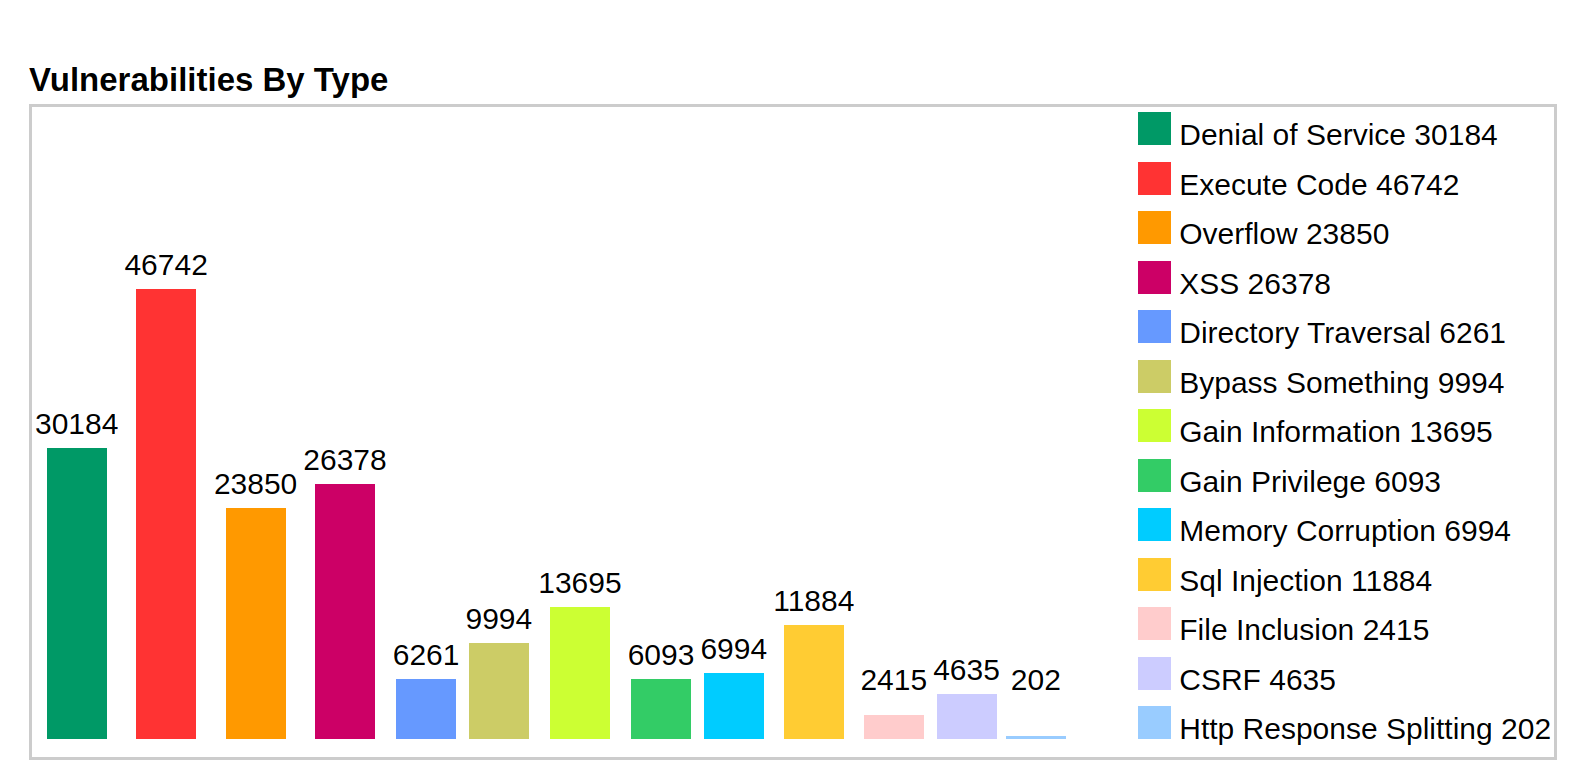
\includegraphics[width=7cm]{./figures/mitre.png}
% \caption{Vulnerabilities by type, classified by MITRE \cite{mitre} }
% \end{figure}

However, it remains to be seen whether regular software developers can use capability-based languages in teams to design applications and the effect of doing so on introduced security vulnerabilities, compared with a library-based approach. To answer this question, we frame the following research questions for the project:

\begin{enumerate}
    \item \textbf{RQ1}: How usable are capability-based languages when designing an architecture?
    \item \textbf{RQ2}: What security vulnerabilities do programmers expose when designing resource-critical objects?  
\end{enumerate}

To answer these questions, we set up a comparative study between two languages - one with object capabilities (Wyvern) and the other with support for capabilities via external libraries (Rust). The two languages were chosen based on the following parameters:

\noindent
\textbf{Reasons to choose Wyvern}
\begin{enumerate}
    \item Provides a capability-based module-system with formalized authority-control \cite{DBLP:journals/darts/MelicherSPA17}. Here, system resources are represented as object capabilities and must explicitly be passed as arguments, limiting access to certain system resources. This feature will help us to design a multi-tiered architecture while controlling security in each layer.
    \item Domain-specific syntax support within the language provides good support for embedding other languages (such as in the case of web development HTML/SQL), so users can have an easier time designing architecture with high safety/security properties.
    \item A potential future scope of the Wyvern project lies in studying the usability and security of Effect Systems in conjunction with capabilities. A comparable language is Koka \cite{leijen2014koka}, but it's effect system does not have a focus on security since it does not support the principle of information hiding. 
    % https://www.cs.cmu.edu/afs/.cs.cmu.edu/Web/Posters/ISRProposal-SE-Document-DMelicher18.pdf
    % TODO: Look into https://doc.lagout.org/science/0_Computer%20Science/1_Principles%20of%20Programming%20Languages/Design%20Concepts%20in%20Programming%20Languages%20%28MIT%2C%202008%29.pdf <- proof-carrying code
\end{enumerate}


\noindent
\textbf{Reasons to choose Rust}
\begin{enumerate}
    \item In terms of choosing a capability library among modern languages, the Rust library was found to be the most stable. (Object-Capabilities in Scala \cite{scalaCaps} was another candidate but the library is currently in beta).
    \item Considered as the most loved language on Stack Overflow \cite{rustLove}, so a strong case for increasing future user adoption rates.
    \item Supports multiple paradigms of programming, such as imperative and functional programming, which increases suitability for getting more users for the study.
    \item Systems language with a strong type system, known to be secure due to ownership, so it would be interesting to see security vulnerabilities arising from using this language.
\end{enumerate}

Our findings are in their preliminary stages. They show that programs designed in Wyvern provided higher security guarantees, and users found that object capabilities provided an easy-to-use yet a secure abstraction layer for critical resource management. However, a lack of tooling for showing appropriate errors or code completion introduced ease of use challenges when writing programs. Informed by these findings, future work is required primarily in designing a more in-depth study to understand the user-centric methods needed to design capability-based languages. Further work also involves classifying security vulnerabilities solved by capabilities and building the necessary static analysis tools/debugging aids in Wyvern to make capabilities more viable as a design choice in programming languages.